\chapter{ Análisis}

\section{ Análisis del Problema}
El principal problema que se plantea solventar es el desarrollo de una API gráfica que sea capaz de ilustrar el funcionamiento de algoritmos de simplificación geométrica. Este desarrollo implica el estudio de las últimas tecnologías y metodologías de programación gráfica, programación orientada a objetos así como de estructuras de datos.\\

Una API es una interfaz de programación de aplicaciones, o su nombre en ingles del que proceden las siglas: \textit{Application Programming Interface}. La API no es más que un software que encapsula una serie de funciones para volver a usarse más adelante favoreciendo la reusabilidad del software y siguiendo los principios de la Ingeniería de Software (\cite{sommervilleSoftwareEngineeringGlobal2016}) además de una documentación sobre como utilizar correctamente dicho software.\\ 


Para solucionar el problema principal se ha dividido el proyecto en dos etapas, la primera consiste en crear un software que muestre al usuario imágenes de objetos 3D generadas a partir de un fichero que define una malla de triángulos según las especificaciones de ``Polygon File Format'', también llamado \textit{render} y la segunda el estudio, implementación y aplicación de algunos algoritmos de simplificación geométrica a mallas que previamente han sido importadas en el render.

\subsection{ Renderizador}
El primer sub-problema al que me enfrento es la de crear un renderizador capaz de mostrar mallas de triángulos en tres dimensiones y que permitan al usuario una visualización cómoda y fácil. Para ello necesito una API gráfica para la generación y manejo de los gráficos y un framework de desarrollo. Un claro ejemplo de render es \texttt{Meshlab} (ver ejenplo \ref{fig:meshlab_presentacion.png}). \texttt{Meshlab} es un software muy avanzado de gráficos pero yo solo me centraré en  cumplir con los requisitos especificados en el capitulo segundo.\\

\begin{figure} %con el [H] le obligamos a situar aquí la figura
	\centering
	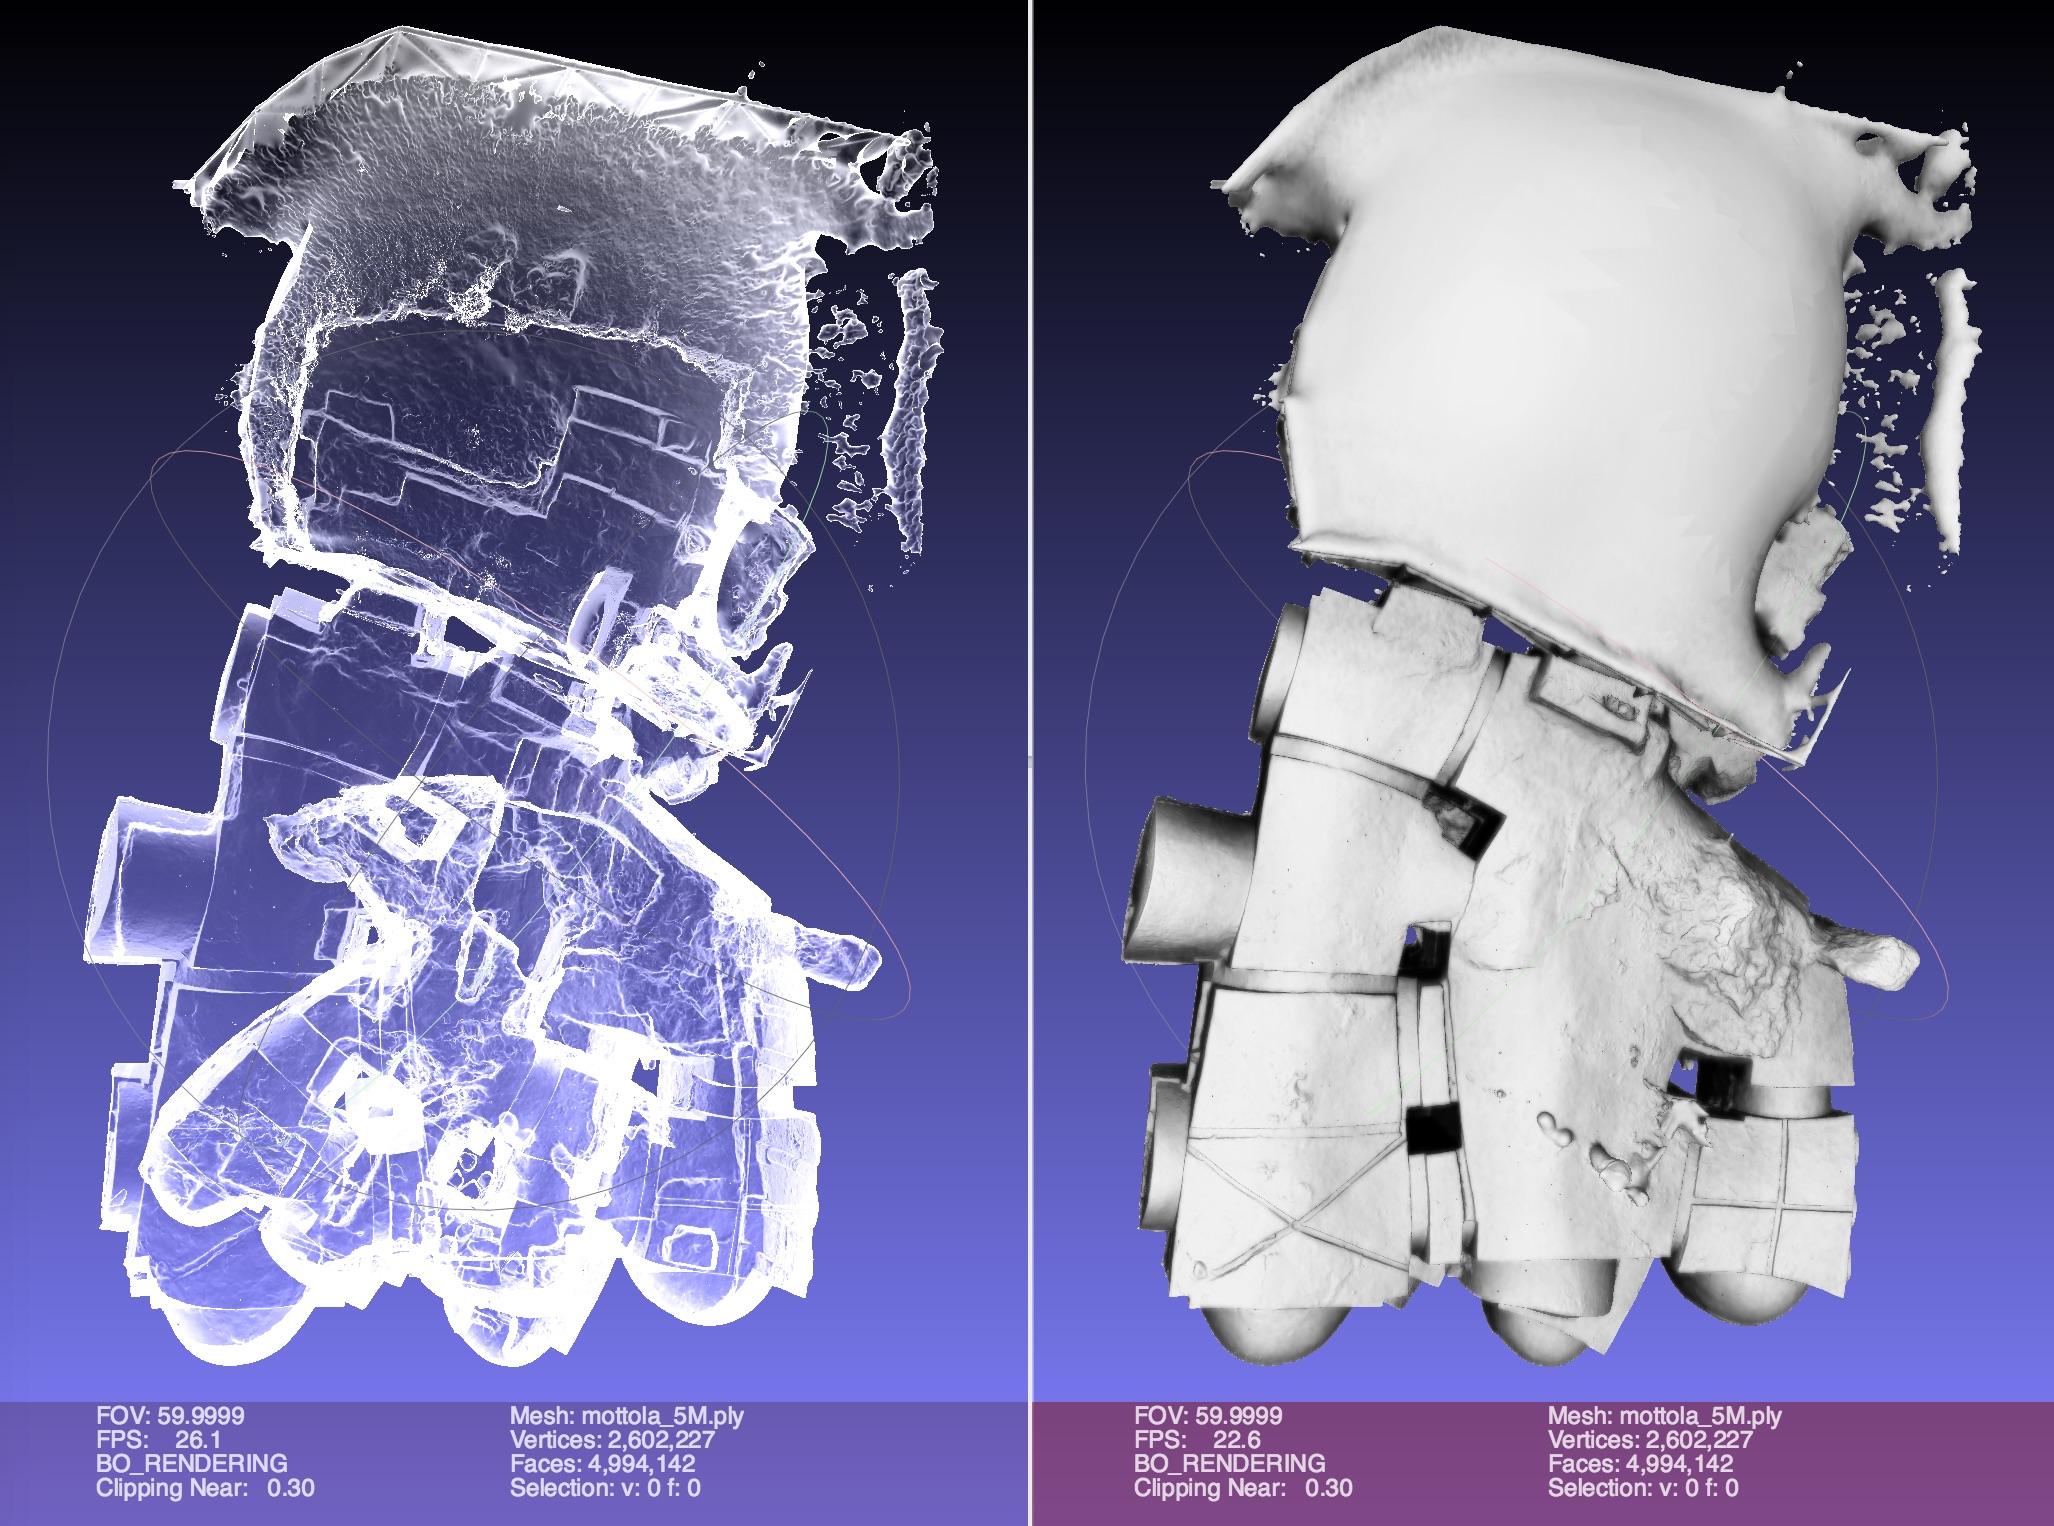
\includegraphics[scale=0.15]{imagenes/Presentation.jpg} 
	\caption{ Imagen renderizada por MeshLab \cite{cignoniMeshLabOpenSourceMesh2008}} \label{fig:meshlab_presentacion.png}
\end{figure}

Para cumplir el primer requisito funcional (\ref{RF1}) se debe de realizar una muy buena gestión de la estructura de datos que almacenará todos los elementos y atributos de la malla de triángulos. Si analizamos con más detalle la malla vemos que está compuesta principalmenete de la geometría y la topología. Como indica Martti Mäntylä \cite{marttimantylaIntroductionSolidModeling}: \textquotedblleft La geometría de un modelo viene dada por las coordenadas de aquellos puntos que están sobre la superficie y la topología de un modelo es cómo se organiza la geometría para dar lugar a una superficie \textquotedblright. De modo que sintetizamos la geometría en los vértices y la topología en las aristas que unen dichos vértices formando la malla triangular. Por tanto para almacenar los vértices usaremos la siguiente estructura:\\

Vértice:

\begin{algorithmic}
\hrule
	\State $Atributos$
	\State \hspace{1cm} $position : 3-Tupla(Real)$
	\State \hspace{1cm} $color : 3-Tupla(Real)$
	\State \hspace{1cm} $halfEdgeIn : HalfEdge[]$
	\State \hspace{1cm} $halfEdgeOut : HalfEdge[]$
	\State \hspace{1cm} $id : Natural$
\hrule
\end{algorithmic}
\vspace*{1cm}

Definiendo en más detalle los atributos:
\begin{itemize}
	\item \textbf{position}: representa las coordenadas X,Y,Z de un vértice en el espacio.
	\item \textbf{color}: indica en en formato RGB de cada vértice.
	\item \textbf{halfEdgeIn}: array de referencias a las semi-aristas aladas que inciden en el vértice.
	\item \textbf{halfEdgeOut}: array de referencias a las semi-aristas aladas que salen del vértice.
	\item \textbf{id}: Entero que identifica al vértice.
\end{itemize}

Para en caso de las aristas, como ya se introdujo en el capitulo 1 pero lo detallaremos más, se ha tomado la decisión de utilizar una estructura más moderna que las aristas normales y son las semi-aristas aladas. Esta decisión está apoyada por las sustanciales mejoras que aporta esta estructura frente a otras. En comparación con la de aristas dirigidas como se dice en el estudio de ``Using generic programming for designing a data structure for polyhedral surfaces'' (\cite{kettnerUsingGenericProgramming1999}) y en ``Directed Edges—A Scalable Representation for Triangle Meshes'' (\cite{campagnaDirectedEdgesScalable1998}) donde se exponen las ventajas, algunas como la facilidad de navegación por la malla. Este aspecto es clave a la hora de aplicar algoritmos de procesado geométrico donde la navegación por la malla es una operación muy utilizada y si una estructura de datos facilita dicha operación en tiempo, facilidad y potencia es una elección muy importante. Es cierto que las aristas aladas son muy parecidas a las semi-aristas aladas a primera vista, pero si se examinan con más detalle se puede observar un problema que ocurre en las aristas aladas. La topología que une dos vértices se orienta en el caso de las aristas dirigidas cómo, una arista que va del vértice $a$ al vértice $b$ con toda la información correspondiente. Además tiene que existir otra arista que vaya del vértice $b$ al vértice $a$ con prácticamente los mismos datos. Lo que ocasiona una repetición de información cuando lo analizamos a nivel global de toda la malla, pues por cada arista se están repitiendo el puntero a las caras adyacentes y las referencias a las aristas anteriores y siguientes, pero en orden contrario. Esta duplicación de información desaparece con las semi-aristas aladas pues al dividir cada arista dirigida en dos una en el mismo sentido y otra con el sentido contrario ya solo se almacena la información justa. Además otra ventaja es que no hace falta comprobar la orientación de la arista puesto que al estar ya dividida en dos, una para cada sentido ya está implícito en cada semi-arista. \\

Ahora es necesario implementar la estructura de semi-aristas aladas y se ha diseñado de la siguiente forma:\\

Semi-Aristas Aladas:
\begin{algorithmic}
	\hrule
	\State $Atributos$
	\State \hspace{1cm} $id : Integer$
	\State \hspace{1cm} $vertexIn : Vertice$
	\State \hspace{1cm} $vertexOut : Vertice$
	\State \hspace{1cm} $face : Cara$
	\State \hspace{1cm} $nextHalfEdge : HalfEdge$
	\State \hspace{1cm} $opositeHalfEdge : HalfEdge$
	\State \hspace{1cm} $previousHalfEdge : HalfEdge$
	\hrule
\end{algorithmic}
\vspace*{1cm}

Los atributos definen lo siguiente:
\begin{itemize}
	\item \textbf{id}: Entero que identifica a la semi-arista alada.
	\item \textbf{vertexIn}: referencia al vértice sobre el que incide la semi-arista.
	\item \textbf{vertexOut}: referencia al vértice del que sale la semi-arista alada.
	\item \textbf{face}: referencia a la cara sobre la que incide.
	\item \textbf{nextHalfEdge}: referencia a la semi-arista siguiente, entendiendo siguiente como la semi-arista que sale del vértice sobre el que incide e incide sobre la misma cara.
	\item \textbf{opositeHalfEdge}: referencia a la semi-arista contraria, es decir, que tiene la misma posición pero la dirección opuesta.
	\item \textbf{previousHalfEdge}: referencia a la semi-arista anterior.
\end{itemize}

Una vez tenemos los vértices y las semi-aristas definidas cómo se van a implementar, el siguiente elemento que surge son las caras. Una cara es una superficie delimitada por tres semi-aristas seguidas que unen tres vértices. Las caras en nuestro caso solo se necesitan para el procesado de mallas, ya que para la renderización nos basta con los vértices y las semi-aristas. Pero para el procesado sí que es necesario guardar cierta información para la navegación de la malla.\\
\newpage
Face:
\begin{algorithmic}
	\hrule
	\State $Atributos$
	\State \hspace{1cm} $id : Integer$
	\State \hspace{1cm} $vertices : Vertice$
	\State \hspace{1cm} $normal : 3-tupla(Real)$
	\hrule
\end{algorithmic}
\vspace*{1cm}

Los atributos definen lo siguiente:
\begin{itemize}
	\item \textbf{id}: Entero que identifica a la cara.
	\item \textbf{vertices}: referencias a los vértices que componen la cara.
	\item \textbf{normal}: normal de la cara.
	
\end{itemize}


\subsubsection{API Gráfica}
En primera instancia se abordó crear el renderizador utilizando la API gráfica de ``Vulkan''  pero la instalación del entorno se complico y se decidió cambiarla por una más conocida y probada como es ``OpenGL''. Los beneficios que aporta Vulkan sobre OpenGL son muchos más que sus desventajas. Se trata de una tecnología nueva, liberada en Febrero de 2016 \cite{KhronosReleasesVulkan2016}, pensada para el  Hardware que hay disponible en el mercado comercial como son: procesadores multi-núcleo, tarjetas gráficas más potentes y con gran capacidad de almacenamiento, etc. Esta premisa es el principal avance con respecto a su antecesor(OpenGL) que al ser una tecnología de los años 90,aunque se ha actualizado pero su base sigue limitada por los planteamientos originales de la época. Vulkan se sostenta en la paralelización de los ``Buffers'' mediante los ``Command Buffers'' \cite{tristanlorachSiggraph2016Vulkan17:36:01UTC}.  De esta forma se aprovechan todos los núcleos del procesador y sus potencia de cálculo para preparación de datos, control logístico de los datos, etc. Reduciendo el cuello de botella que se producía entre la CPU y el procesador gráfico de la tarjeta gráfica. Esto se traduce en una mejora de las prestaciones de forma notable. Los fabricantes de tarjetas gráficas \texttt{PowerVR}, \texttt{Imagination}, han realizado varias comparaciones \cite{VulkanVsOpenGL2017a} y demostrando el mejor control de los núcleos de la CPU y evitando la saturación de uno de ellos y por consiguiente el cuello de botella que se produce. \\

Como contra por parte de Vulkan el control de los ``Command Buffers'' ha tenido que bajarse el nivel de abstracción dejando al programador más responsabilidad de programación y más compleja dicha tarea.


Por estos motivos se decidió seleccionar Vulkan como principal API gráfica, pero al ser una tecnología nueva y con poco uso fuera del ámbito industrial complicó mucho la instalación y configuración en el entorno de trabajo, como se ha explicado en apartados anteriores.\\

Así pues se toma como API gráfica OpenGL, que nos permite el control del cauce gráfico para mostrar objetos en la pantalla. 
El proceso para la renderización de la malla se realiza de la siguiente forma en el cauce gráfico.\\

Lo primero es la configuración inicial de OpenGL para la creación de una escena, una escena es el espacio virtual que se asemeja a una escena de una película. Donde está compuesta por objetos que se colocan de una forma concreta, la iluminación y la cámara que capta la imagen. El concepto es el mismo pero en un entorno virtual, se requiere un espacio donde se alojan los objetos, en nuestro caso son las mallas de triángulos, las iluminación, que ya nos la provee OpenGL una simulación, y por último nos ofrece distintos tipos de cámaras para construir la escena por completo.\\

Como ya hemos dicho todos los objetos se alojan en la escena, pero entendemos por alojar a que todos los objetos están posicionados en la escena con una posición global, la cual define su posición con respecto a las coordenadas de la escena y unas coordenadas locales a cada objeto. De esta forma podemos tener agrupados distintos tipos de objetos para formar otros más complejos y compuestos, como por ejemplo juntar  una malla con forma de coche y un objeto cámara que esté relacionado con el coche y así que cuando se mueva el coche se mueva la cámara con él. Esta forma de asociar unos objetos con otros es muy útil y permite un gran control para construir escenas muy grandes y complejas como deseemos.

\subsubsection{ Shaders}

Los ``Shaders'' (\cite{LearnOpenGLShaders} y \cite{ShaderOpenGLWiki}) son programas ejecutados en el GPU con un lenguaje propio y normalmente suelen ser pequeños y de uso concreto. Se dividen en dos, los \texttt{vertex Shaders} y los \texttt{fragment Shaders}. Cada uno tiene una funcionalidad bien definida. Trabajando entre todos por fases y produciendo una imagen final adaptada a la pantalla que será la que se muestre finalmente.El flujo simplificado sería el que se muestra en la figura \ref{fig:pipeline.png} donde se va generando la imagen que se mostrará por pantalla poco a poco. \\

El \texttt{vertex Shader} (\cite{VertexShaderOpenGL}) es el primer paso dentro de los shaders y se encarga de la generación de la geometría y el procesamiento a nivel de vértices. Recibe como entrada un array de vértices entre otros atributos. Los procesa aplicandoles las transformaciones que se le han indicado generando como resultado la geometría en su posición final.\\


El \texttt{fragment Shader} (\cite{FragmentShaderOpenGL}) recibe como entrada la salida del verter shader. Es el encargado de rasterizar la imagen final y pasarla a una matriz para poder representarla en un monitor.Esto requiere aplicar las texturas y materiales indicadas en los buffers dedicados a ello. Además de los efectos que se deseen aplicar.\\


\begin{figure} %con el [H] le obligamos a situar aquí la figura
	\centering
	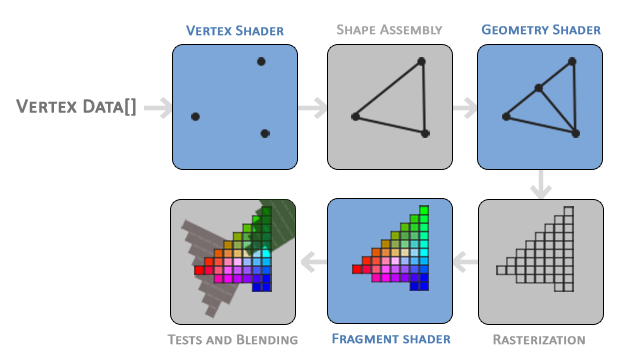
\includegraphics[scale=2]{imagenes/pipeline.png} 
	\caption{ Fases del Shader, imagen de \url{https://learnopengl.com/Getting-started/Hello-Triangle} } \label{fig:pipeline.png}
\end{figure}


\begin{figure} %con el [H] le obligamos a situar aquí la figura
	\centering
	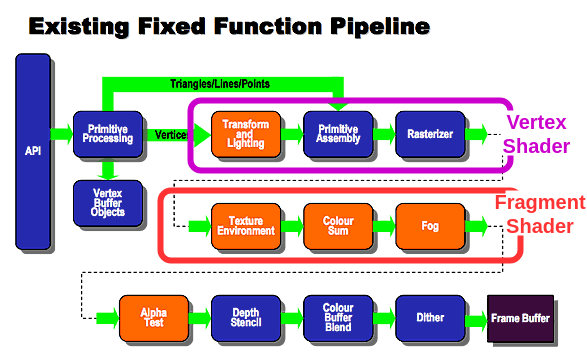
\includegraphics[scale=0.7]{imagenes/opengles_1x_pipeline.png} 
	\caption{ Flujo completo de los Shaders, imagen de \url{http://resumbrae.com/ub/dms423/18/} } \label{fig:opengles_1x_pipeline.png}
\end{figure}


Los \texttt{buffers}  son los encargados de alojar en memoria de la GPU datos para su posterior procesamiento en los Shaders, como he explicado antes. Las GPUs están especialmente diseñadas para optimizar el procesamiento en paralelo de múltiples datos con la misma función,  por ello OpenGL nos ofrece una serie de tipos de Buffers para cargar los datos en bloques grandes de forma paralela. OpenGL posee ya definidos distintos tipos para cada tipo de propósito. Los primeros son los \texttt{``Vertex Buffer Object''} (VBO), destinados a guardar vértices así como sus atributos, como pueden ser el color de cada vértice. Luego están los \texttt{``Vertex Array Object''} (VAO), son muy parecidos a los VBO, pero permiten guardar uno o muchos VBO entre otros tipos de buffers como los EBO por ejemplo. Formando así una estructura más compleja dentro de la Memoria de la GPU con toda la información relativa a un objeto. Otro tipo son los \texttt{``Element Buffer Object''} (EBO) que definen como se construye el elemento en cuestión con los vértices ya almacenados, se puede decir que definen la topología del elemento. En la figura \ref{fig:dia_buffers.png} se puede observar más claramente un ejemplo de uso de los buffers, donde los VBO se utilizan para asignarle a una figura su geometría y el color de cada vértice y el EBO se especifica los indices. Los índices son un array que contiene $n$ grupos de tres enteros, donde cada grupo indica a tres vértices, mediante la posición del array de vértices ,que componen un triángulo y $n$ es el número de triángulos que tiene el elemento. 

Es el VAO el que se manda por el el shader para generar la imagen siguiendo el esquema de la figura \ref{fig:opengles_1x_pipeline.png}.


\begin{figure} %con el [H] le obligamos a situar aquí la figura
	\centering
	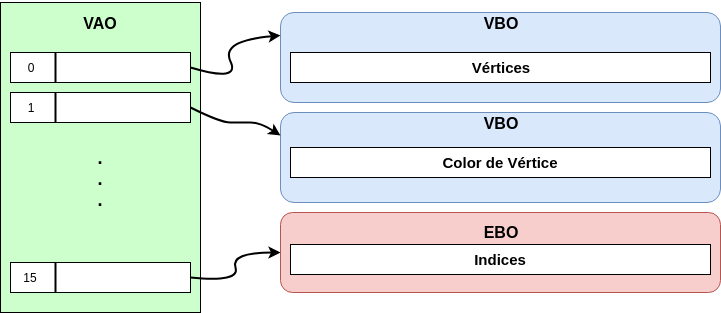
\includegraphics[scale=0.5]{imagenes/dia_buffers.png} 
	\caption{ Diagrama de funcionamiento de los Buffers VAO, VBO y EBO } \label{fig:dia_buffers.png}
\end{figure}


\subsubsection{1.1.1.2 Cámara}
La cámara es un elemento virtual en OpenGL, puesto que no existe un objeto tal y como entendemos la cámara: objeto que permite captar imágenes, pero sí se puede simular un comportamiento parecido (como nos enseñan en LearnOpenGL \cite{LearnOpenGLCamera}). OpenGL nos ofrece una serie de herramientas para esta simulación. Lo primero es que no tenemos un objeto que capte imágenes de la escena, pero si tenemos como una ``ventana'' por la cual podemos mirar. Esta ``ventana'' está en una posición fija en las coordenadas globales de la escena. Esto obliga a que para mover la cámara utilicemos la matriz de transformaciones, que es la que se aplica a todos todos los elementos en bloque. De esta forma si movemos el mundo con todos los objetos da la sensación de que la cámara se está moviendo. Por lo tanto para posicionar y que mire a donde queremos es necesario aplicar ciertas transformaciones a la matriz transformación.\\

Lo primero es posicionar la cámara en el espacio, y para ello es necesario crear una matriz con transformaciones que se añadirá a la matriz de transformación. Para posicionar la cámara se utiliza el principio de ejes de la aviación (\cite{AircraftPrincipalAxes2018}), que a su vez están basados en los ángulos de Euler (\cite{EulerAnglesWolfram}) comúnmente conocidos por ``Yaw, pitch and roll'' en la figura \ref{fig:Yaw_Axis_Corrected.png} se puede apreciar un ejemplo sobre un modelo de un avión, además de forma visual es más fácil entender en que consiste este principio. Consiste en la posición de tres ejes que hacen referencia a los ejes cartesianos en el espacio 3D, $X, Y y Z$ de esta forma es posible orientar la cámara y posicionarla donde se desee mediante la definición de los tres vectores unitarios y unas coordenadas de posición. El primer vector es el simbolizado como una $R$ y hace referencia al eje $X$ y en el modelo de Euler al eje ``Pitch'', otro vector es el vector ``Up'' simbolizado con $U$ y en el modelo de Euler llamado ``Yaw'' y por último el vector dirección, $D$, en Euler es el eje ``Roll''.\\

\begin{figure} %con el [H] le obligamos a situar aquí la figura
	\centering
	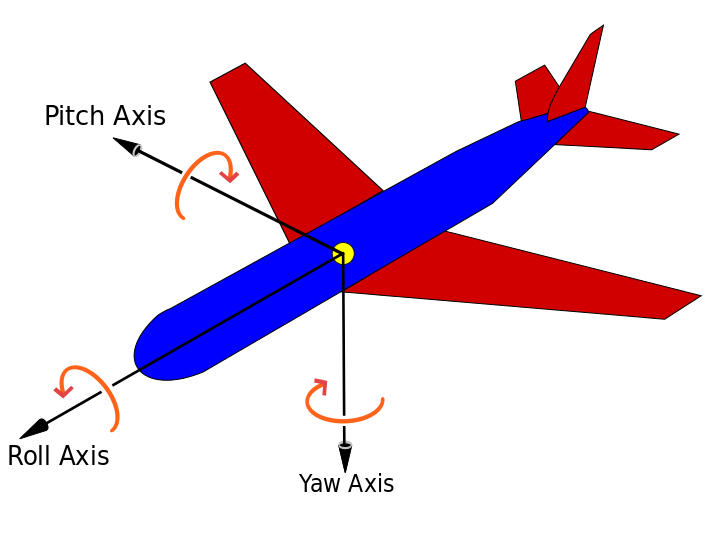
\includegraphics[scale=0.5]{imagenes/Yaw_Axis_Corrected.png} 
	\caption{ Ejes Yaw, Pitch and Roll sobre un modelo de un avión, fuente \cite{AircraftPrincipalAxes2018}} \label{fig:Yaw_Axis_Corrected.png}
\end{figure}

Combinando todos los elementos tenemos la cámara ``posicionada'' y apuntando a donde deseemos mediante la siguiente matriz de transformación que se aplicará a la matriz de transformación global. \\  
\[ 
	M=
	\begin{bmatrix}
		R_{x} & R_{y} & R_{z} & -P_{x}\\
		U_{x} & U_{y} & U_{z} & -P_{y}\\
		D_{x} & D_{y} & D_{z} & -P_{x}\\
		0 & 0 & 0 & 1 
	\end{bmatrix}
\]

Una vez tenemos la cámara posicionada y apuntando hacía donde queremos, ahora necesitamos definir otro aspecto importante de la cámara, la ``lente''. La lente de una cámara es quién le da las propiedades de cuanto capta exactamente la cámara del mundo. Igual que el objetivo de una cámara real que define el ángulo que es capaz de capturar, la calidad y la distancia máxima que es capaz de captar, en OpenGL existen propiedades que son semejantes que de encapsulan en el \texttt{frustum}. Como bien se explica en la guía de la asignatura de Informática gráfica (\cite{franciscojaviermelerorusGuiaAsignaturaInformatica2016}) el frustum es ``[...] la parte de la escena virtual que será considerada a la hora de generar la imagen 2D.'', frustum también es una forma geométrica que se obtiene cortando una pirámide de forma paralela a la base, en nuestro caso será de una base cuadrada.  Tal y como se comentó anteriormente OpenGL genera una escena virtual pero por temas de optimización no se renderiza toda ella, solo lo que se va a mostrar, por lo tanto es muy importante definir bien el frustum, ya que solo la parte de la escena que esté contenida en el frustum se renderizará. Para definir el frustum OpenGL posee los siguientes parámetros:

\begin{itemize}
	\item Near, distancia de la cámara a la cara más cercana a la cámara.
	\item Far, distancia de la cámara a la cara más lejana a la cámara.
	\item Bottom, distancia del centro de la cara a distancia Near, hasta la arista inferior del frustum.
	\item Top, distancia del centro de la cara a distancia Nea, hasta la arista superior del frustum.
	\item Right, distancia del centro de la cara a distancia Near, hasta la arista derecha del frustum.
	\item Left, distancia del centro de la cara a distancia Near, hasta la arista izquierda del frustum.
\end{itemize}

OpenGL con estos parámetros ya genera el frustum sobre la escena, se puede ver más claro en la figura \ref{fig:frustum.png}. Además al ser una escena virtual es posible modificar la perspectiva de captación de la imagen de la cámara, teniendo además de la vista en perspectiva la vista ortogonal.

\begin{figure} %con el [H] le obligamos a situar aquí la figura
	\centering
	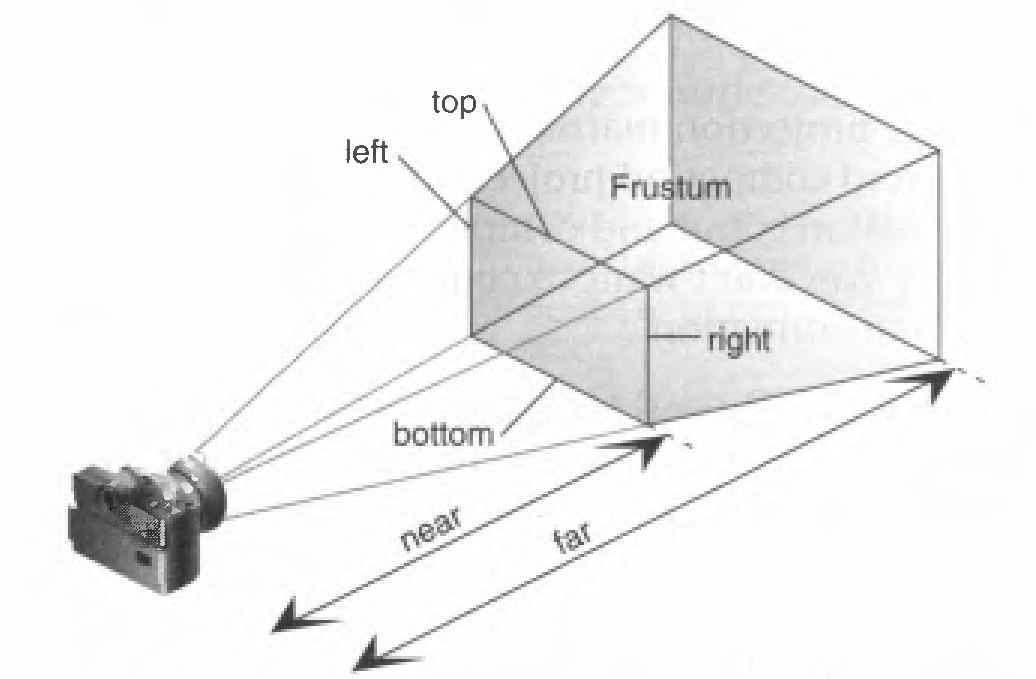
\includegraphics[scale=1]{imagenes/frustum.png} 
	\caption{ Frustum y los parámetros que los define.} \label{fig:frustum.png}
\end{figure}

\subsubsection{1.1.2 Framework de trabajo}

El proyecto se ha realizado utilizando el framework de \textit{``QT''}, en concreto, la versión \texttt{QT 5.10.1}. Se ha optado por este framework por sus elementos que ya contemplan la programación de gráficos con canvas diseñados especialmente para las API's gráficas OpenGL y Vulkan \cite{GraphicsQt11}. Además de contener una gran cantidad de clases especializadas en vectores, matrices y estructuras de datos ya implementadas. También cuenta con una gran disponibilidad independiente de la plataforma de desarrollo y la IDE de desarrollo es muy fácil de utilizar. Por estas razones se ha seleccionado \texttt{QT} como el framework de desarrollo para este proyecto.


\subsubsection{1.1.3 Entrada de Usuario}
Uno de los requisitos del sistema es la interacción con el usuario, así pues se ha decidido que el usuario pueda navegar por la escena generada para que así pueda observar completamente la malla 3D. El método de navegación consiste el movimiento de la cámara mediante el teclado. Utilizando el teclado el usuario podrá variar la posición y los elementos que definen el punto objetivo de la misma. Permitiendo que el usuario pueda elegir la vista que desee, y mejorando por consiguiente la experiencia de usuario.

\subsubsection{1.1.4 Polygon File Format (.ply)}

El formato \texttt{PLY} fué descrito por \textit{Greg Turk} en el artículo \cite{turkPLYPolygonFormat}, donde por primera vez se definía de forma pública y de forma abierta una manera de representar mallas de polígonos en ficheros de texto de forma sencilla, precisa y completa. Con este formato se puede especificar las partes de una malla que se deseen, desde solo la geometría y la topología, hasta el coeficiente de refracción. Siguiendo unas palabras reservadas y un orden se puede especificar cualquier elemento, siempre dentro del ámbito de las mallas poligonales. No es de extrañar que se haya convertido prácticamente en un estandar dentro del mundo de los gráficos, ya que al ser independiente de cualquier organismo privado no está sujeto al beneficio personal.\\

El formato de un fichero PLY sigue la siguiente estructura:

\begin{itemize}[label={--}]
	\item Cabecera: Se especifica el contenido del fichero, como su formato, número de elementos, propiedades de los elementos, etc.
	\item Lista de vértices: un listado de los vértices, en cada línea se pone un vértice. Además si se ha especificado alguna propiedad del vértice en la cabecera (como el color de vértice) se añade a continuación, el color sería en formato RGB, en la misma línea.
	\item Lista de caras: Listado que define cada una de las caras, las caras siguen el formato de indexación de vértices. Cada cara se define en un línea, así como sus posibles propiedades de cada cara.
	\item Lista de otros elementos: como pueden ser la luz ambiental que posee el objeto o cualquier otra propiedad. 
\end{itemize}

\subsection*{1.2 Procesado Geométrico}
El procesado geométrico es la segunda parte y principal del proyecto. El procesado geométrico permite la manipulación de la malla para conseguir transformarla en muchos sentidos y es un área cada vez más grande y donde más gente investiga. El procesado geométrico se puede dividir en varios campos (\cite{CS468GeometryProcessing} y \cite{GeometryProcessingCourse}).

\begin{itemize}
	\item \textbf{Captación:} consiste en generar mallas de polígonos perfectamente formadas a partir de un modelo real. En este campo se encuentran los escáneres láser, la tomografía que se usa en la sanidad y ha permitido realizar muchos avances.
	\item \textbf{Análisis:} realiza un entendimiento de la malla y la comprensión de los elementos y propiedades de la que la construyen. En la arqueología y en la ingeniería se utiliza para comprobar las propiedades físicas de los materiales mediante simulación de modelos en vez de contar con el objeto real.
	\item \textbf{Manipulación:} modifica la malla, alterando sus propiedades, la geometría, topología, etc para conseguir variaciones de la malla. En este ámbito se encuentra los modeladores 3D, que se utilizan en los videojuegos y cine, donde permiten a una figura ya creada moverle partes de forma natural sin tener que re-dibujala, también se utiliza en el estudio de objetos antiguos para la regeneración de un objeto completo a partir de partes de un objeto (\cite{meleroInteractive3DReconstruction2003}).
	
\end{itemize}

Pero el campo sobre el que trabaja este proyecto es la manipulación. Me centraré en la parte de simplificación de una malla. La simplificación de mallas es una parte importante de la manipulación, permite generar una malla parecida a la original pero con menos fidelidad y por tanto con menos elementos, dando así como resultado una malla más fácil de cargar y renderizar en vídeo. La renderización de mallas hiper realistas es un problema por el hardware actual. En el mundo de los videojuegos se exponen miles de elementos en la escena y el objetivo es que todos reaccionen en tiempo real a los eventos del jugador. Pero esto tiene un coste de computación muy elevado que a día de hoy es inasumible. Por ello se buscan métodos de mejorar el tiempo de renderizado sin que el usuario note perdida de calidad de la escena. Una de las técnicas utilizadas es el \texttt{Level Of Details}, o nivel de detalle, que consiste en tener varias mallas o modelos de un objeto con diferentes grados de calidad o exactitud con el original, de este modo se puede cargar  objetos con un tercio de los triángulos originales cuando se sitúa en el fondo de la escena y con forme nos vamos acercando al objeto se cambia por otro con más triángulos hasta llegar al modelo original. Un ejemplo gráfico es el de la figura \ref{fig:polygon-reducer-lod-1.png}, donde se ve un conejo con distintos grados de detalle y triángulos, y aunque a primera vista puede apreciarse muy claramente las diferencias si las exponemos a una cierta distancia como en la figura \ref{fig:polygon-reducer-lod-2.png} se puede ver claramente como realmente parece la misma figura.\\

Para esta técnica de reducción de triángulos se pueden aplicar distintos métodos para conseguir mallas con menos exactitud, como por ejemplo el re-modelado, donde un artista reduce los triángulos a mano o por el contrario de forma automática mediante algoritmos. En este momento entra el procesado de mallas y la simplificación geométrica. Este campo como ya se ha comentado anteriormente existen varios algoritmos que permiten reducir la cantidad de triángulos según varios criterios. En nuestro caso nos centramos en el ``decimation''.

\begin{figure} %con el [H] le obligamos a situar aquí la figura
	\centering
	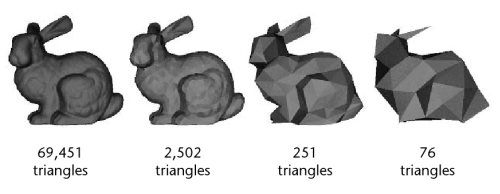
\includegraphics[scale=0.8]{imagenes/polygon-reducer-lod-1.jpg} 
	\caption{ Distintos grados de exactitud y cantidad de triángulos de una malla, fuente \url{http://polygon-reducer.pc-guru.cz/reducing-level-of-detail?skin=tisk}} \label{fig:polygon-reducer-lod-1.png}
\end{figure}

\begin{figure} %con el [H] le obligamos a situar aquí la figura
	\centering
	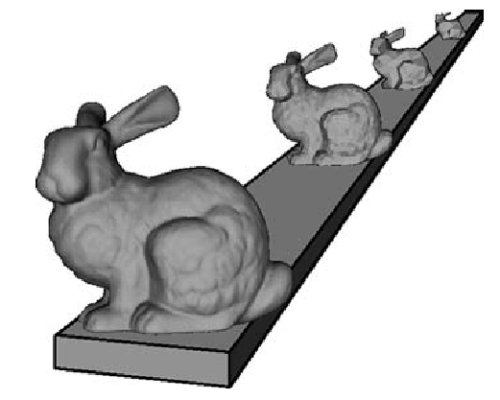
\includegraphics[scale=0.5]{imagenes/polygon-reducer-lod-2.jpg} 
	\caption{ Level of detail en práctica, fuente \url{http://polygon-reducer.pc-guru.cz/reducing-level-of-detail?skin=tisk}} \label{fig:polygon-reducer-lod-2.png}
\end{figure}

\newpage
\subsubsection*{1.2.1 Decimation}
El algoritmo de decimation (\cite{OpenMeshMeshDecimation} y \cite{mirelaben-chenCS468GeometryProcessing}) nos indica una forma de simplificar una malla para que a partir de un porcentaje de error nos genera otra malla con dicho error sobre la malla original. Entendiendo el error de una cara como la sumatoria de los ángulos que forman las normales de cara de las caras adyacentes con respecto a la normal de cara de la propia cara. En la figura \ref{fig:error_decimation.png} para calcular el error de combinar la cara $A$ y la cara $B$ tenemos la cara $A$ y la cara $B$ y para calcular el error que produce que calcular la sumatoria de los ángulos de las normales de cara de las caras $A,B,C,D,E$ y ese sería el error que se produce. De esta forma si dos caras son paralelas el error que produce al combinarlas es de $0$ pero si son perpendiculares es un error de $1.41$, siempre en radianes, en la imagen solo se muestra el ángulo $\alpha$ pero habría que calcularlo con todas las demás caras.\\


\begin{figure} %con el [H] le obligamos a situar aquí la figura
	\centering
	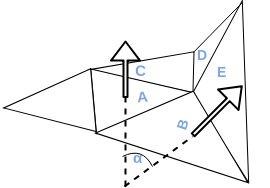
\includegraphics[scale=1]{imagenes/error_decimation.png} 
	\caption{ Ángulo que forman dos normales de cara.} \label{fig:error_decimation.png}
\end{figure}


Una vez calculado el error de combinar todas las caras con sus adyacentes, cogemos la que produce menos error y la combinamos, para combinar dos caras se utiliza el método de collapse, que explico en el siguiente apartado.\\

Existen varias formas de aplicar el método de decimation, la más usual es por aplicación incremental, es decir, se calcula la lista de caras con menos error si se combinarán y se va sacando de la lista cada elemento, se aplica el método de combinado y se actualizan los valores de la lista de errores, puesto que la combinar dos caras las caras adyacentes cambian el error que producen su combinación y posteriormente se analiza si se ha llegado a la tasa objetivo y en caso negativo se vuelve a lanzar, así hasta que se consigue la tasa objetivo.


\subsubsection{ Collapse}

La operación de colapsar dos vértices consiste en dado una semi-arista, colapsar el vértice de origen en el vértice destino. Esta operación requiere de un control de los elementos implicados pues tiene ciertas características que debe mantener. La librería de \texttt{OpenMesh} (\cite{OpenMeshBasicOperations}) se explica cómo realizar esta operación y las medidas a tener en cuenta, además de ilustrar el proceso. En la figura \ref{fig:meshcollapse.png} se puede apreciar el antes y después de aplicar el proceso de collapse a una semi-arista o a su opuesta.\\

\begin{figure} %con el [H] le obligamos a situar aquí la figura
	\centering
	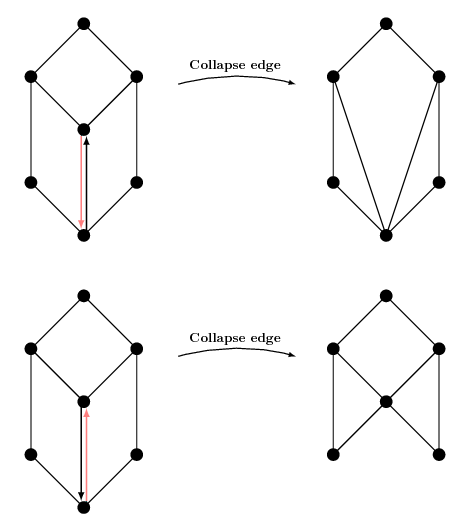
\includegraphics[scale=0.8]{imagenes/meshcollapse.png} 
	\caption{Antes de después de aplicar el método de collapse, la dirección de colapse es la semi-arista roja, fuente \url{https://www.openmesh.org/media/Documentations/OpenMesh-7.0-Documentation/a03935.html}} \label{fig:meshcollapse.png}
\end{figure}

El algoritmo de collapse, tiene que mantener la forma de la malla, es decir, que no puede crear agujeros, ni estructuras de vértices T. Tal y como de explica en la presentación sobre los problemas de las mallas de la universidad de Princeton (\cite{FrequentMeshProblems}) los vértices T (figura de un vértice T )pueden causar muchos problemas a la hora de analizar la malla o aplicarle algoritmos, el propio algoritmo de decimation o collapse requiere para un correcto funcionamiento que la malla fuente esté libre de este tipo de estructura. Los vértices T, rompen la estructura de todos los demás, pues ya no todas las caras contiene a únicamente tres vértices, si no que ahora esté número es desconocido a priori y puede variar cada vez que apliquemos una transformación. Otras características a tener en cuenta y que son altamente recomendables es que sea una malla \texttt{2-manifolds}, como se explica Daniel Müllner en  \cite{2manifoldsManifoldAtlas}, donde las caras están orientadas, no posee vértices T y la superficie no puede cortarse a sí misma. 	

\begin{figure} %con el [H] le obligamos a situar aquí la figura
	\centering
	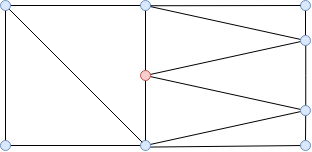
\includegraphics[scale=0.8]{imagenes/T_vertice.png} 
	\caption{Vértice T (de color rojo), frente a vértices normales (color azul)} \label{fig:T_vertice.png}
\end{figure}